
\begin{chapterIntro}
	This section discusses the most relevant components and backends in technical detail.
	For every component listed, the 4+1 view is described (refer to \Cref{sec:about 4+1}).
	The components and backends are ordered according to their position within the I/O stack from the top (application) to bottom (backend).

	\Cref{component: scheduler} discusses the scheduling component that breaks down incoming read and write requests into subsequent requests to create or receive multiple fragments.
	The scheduler relies on a layout component to create a set of domain filling subrequests which is discussed in \Cref{component: layout}.
	In most cases, an application will not interface directly with the ESDM middleware but through a standard frontend.
	\Cref{frontend: hdf5 + mpi} introduces an HDF5 frontend and also discusses how message passing via MPI is realised outside of the ESDM.
	\Cref{frontend: fuse} addresses legacy interfaces using FUSE to expose data sets via configurable virtual file systems.

	It follows the discussion of multiple backends.
	In particular, \Cref{backend: posix} discusses a POSIX backend to allow for interactions with parallel file systems.
	Object storage backends for Mero (see \Cref{backend: mero}) and WOS (see \Cref{backend: wos}) are discussed,
	Besides data backends, also pure metadata backends are possible allowing to use of existing software stacks that are typically also residing on some storage backend themselves.
	\Cref{backend: mongo} describes MongoDB bases metadata backend.
\end{chapterIntro}



%%%%%%%%%%%%%%%%%%%%%%%%%%%%%%%%%%%%%%%%%%%%%
\section{Scheduling Component}
\label{component: scheduler}


I/O requests handled by the ESD middleware are received via the ESDM interfaces as they are described in \Cref{sec: viewpoints/logical/semantics}.
In most cases, these requests must collect additional information / identify multiple fragments to fulfil a request.
The ESDM scheduler is responsible to progress potentially operations, coordinate requests, and invoke the appropriate handlers.
In particular, the scheduler will consult the layout component to determine which fragments to create or use and which storage backends to use.
For a discussion of the decision process for a mapping of a I/O request to backends refer to \Cref{component: layout} on the layout component.


%%%%%%%%%%%%%%%%%%%%%%%%%%%%%%%%%%%%%%%%%%%%%%
\subsection{Logical View}

\begin{figure}
	\centering
	\includegraphics[width=\linewidth]{esdm-components/scheduler/logical.eps}
	\caption{Logical view to the ESDM scheduling component.
	Applications issue requests that are then handled and delegated by the Scheduler to other components.}
	\label{fig:esdm scheduler logical view}
\end{figure}

The scheduling component has two core responsibilities:

\begin{enumerate}
	\item Accept incoming operations from the ESDM Interface and delegate them to handlers possibly in separate threads.
	\item Coordinate the progressing of complex operations and the response/completion of the operations.
\end{enumerate}

In \Cref{fig:esdm scheduler logical view}, the relation of the scheduling component (scheduler) to the rest of the ESDM architecture is illustrated.
An application will issue a request which is queued to the scheduler for consideration.
The scheduler will delegate the request to the layout component which will also consult a performance model to make a decision (refer to \Cref{component: layout} for details).
The resulting operations to internal objects (fragments) may then require a number of requests to various ESDM backends.
These subsequent operations are also coordinated by the Scheduler.




%%%%%%%%%%%%%%%%%%%%%%%%%%%%%%%%%%%%%%%%%%%%%%
\subsection{Process View}

\begin{figure}
	\centering
	\includegraphics[width=\linewidth]{esdm-components/scheduler/process.eps}
	\caption{Process view to the ESDM scheduling component. Applications should when possible issue I/O asynchronously. In either situation the ESDM scheduler may execute multiple threads in parallel to gather or flush fragments to the backends or make a layout decision.}
	\label{fig:esdm scheduler process view}
\end{figure}

The scheduling component is responsible for the bulk of concurrency within the ESDM.
Requests arrive and have to be dispatched to appropriate handlers such as the layout component or a ESDM backend.
This approach is necessary so the ESDM remains responsive as new requests arrive and because it considerably can speed up the reconstruction/flushing of requested views.
\Cref{fig:esdm scheduler process view} provides a overview to active and waiting process as requests are being handled by the ESDM. Notice that Process 1 handles a asynchronous request which allows the application to continue computation, while Process 2 depicts the synchronous case.
In both cases the ESDM will try to perform the domain reconstruction concurrently.


%%%%%%%%%%%%%%%%%%%%%%%%%%%%%%%%%%%%%%%%%%%%%%
\subsection{Physical View}

\begin{figure}
	\centering
	\includegraphics[width=\linewidth]{esdm-components/scheduler/physical.eps}
	\caption{Physical view to the ESDM scheduling component. The scheduler is only active within the application process.}
	\label{fig:esdm scheduler physical view}
\end{figure}


An application may be spread out across many nodes and on each node have multiple running processes.
Each running process that is using ESDM as a scheduling component running as is illustrated in \Cref{fig:esdm scheduler physical view}.
Within ESDM, only the scheduler starts threads.
The ESDM scheduler does not directly expect any modifications or prerequisites from the storage system, but changes to the configuration of the storage system should be reflected in the site configuration.

%
%%%%%%%%%%%%%%%%%%%%%%%%%%%%%%%%%%%%%%%%%%%%%%%
%\subsection{Development View}
%
%\begin{figure}
%	\centering
%	\includegraphics[width=\linewidth]{esdm-component/scheduler/development.eps}
%	\caption{}
%	\label{fig:esdm scheduler development view}
%\end{figure}
%
%\Cref{fig:esdm scheduler development view}
%
%


%%%%%%%%%%%%%%%%%%%%%%%%%%%%%%%%%%%%%%%%%%%%%
\clearpage
\section{Layout Component}
\label{component: layout}

The layout component is responsible for finding a mapping to storage that takes into account information that are available through the conceptional and logical views to the data.
In addition, this section addresses some aspects that explain how the mapping is driven by performance models and the site configuration.


%%%%%%%%%%%%%%%%%%%%%%%%%%%%%%%%%%%%%%%%%%%%%%
\subsection{Logical View}

\begin{figure}
	\centering
	\includegraphics[width=\linewidth]{esdm-components/layout/logical.eps}
	\caption{An application that is using ESDM interfaces through the ESDM API (which in many cases maybe only read/write calls). Eventually the scheduling component has to consult the layout component which is responsible for returning a list of Fragments which have to be read or written. To provide this list the performance model is used which in turn queries the available backends and the site configuration for an estimate.}
	\label{fig:esdm layout logical view}
\end{figure}

The layout component is invoked by the ESDM scheduler to break down incoming requests into fragments that are beneficial from a data access and storage perspective.
The layout components responsibilities in more detail include the following:

\begin{itemize}
	\item map (e.g., a domain) to fragments
	\item where to save new/additional/replica fragments?
	\item time estimates for reading a fragment (e.g., a callback per backend and configuration provided)
	\item time estimates for writing a fragment, in particular find a domain mapping
\end{itemize}

\Cref{fig:esdm layout logical view} illustrates the embedding of the layout component into the larger ESDM architecture.
To find a mapping an important factor is the performance of the individual backends, which requires to know which backends are available.
\Cref{sec:layout/logical/init} describes the initialization process that loads the site configuration.
Storage backends feature wildly different performance characteristics, which is why the ESDM features an abstract performance model that queries the individual ESDM backends to provide performance estimates which may also depend on the data structure of the request.
\Cref{sec: layout/logical/decision} describes the performance model and decision process in more detail.

\subsubsection{Initialization of the Layout/Performance Model}
\label{sec:layout/logical/init}

The layout decision requires knowledge of the available backends.
The ESDM assumes a machine-friendly site configuration to be available.
The site configuration includes a list of available backends for which the ESDM on initialization loads.
\Cref{fig:esdm layout initialisation} shows a UML sequence diagram of the ESDM initialisation process.

\begin{enumerate}
	\item Application/Library: calls ESDM initialisation
	\item ESDM:
	\begin{enumerate}
		\item reads configuration file
		\item discovers and loads available backends + plugins + backend performance model
		\item available backends are announced to the ESDM performance model for consideration
	\end{enumerate}
	\item After successful initialization control is returned to the calling application/library.
\end{enumerate}

\begin{figure}
	\centering
	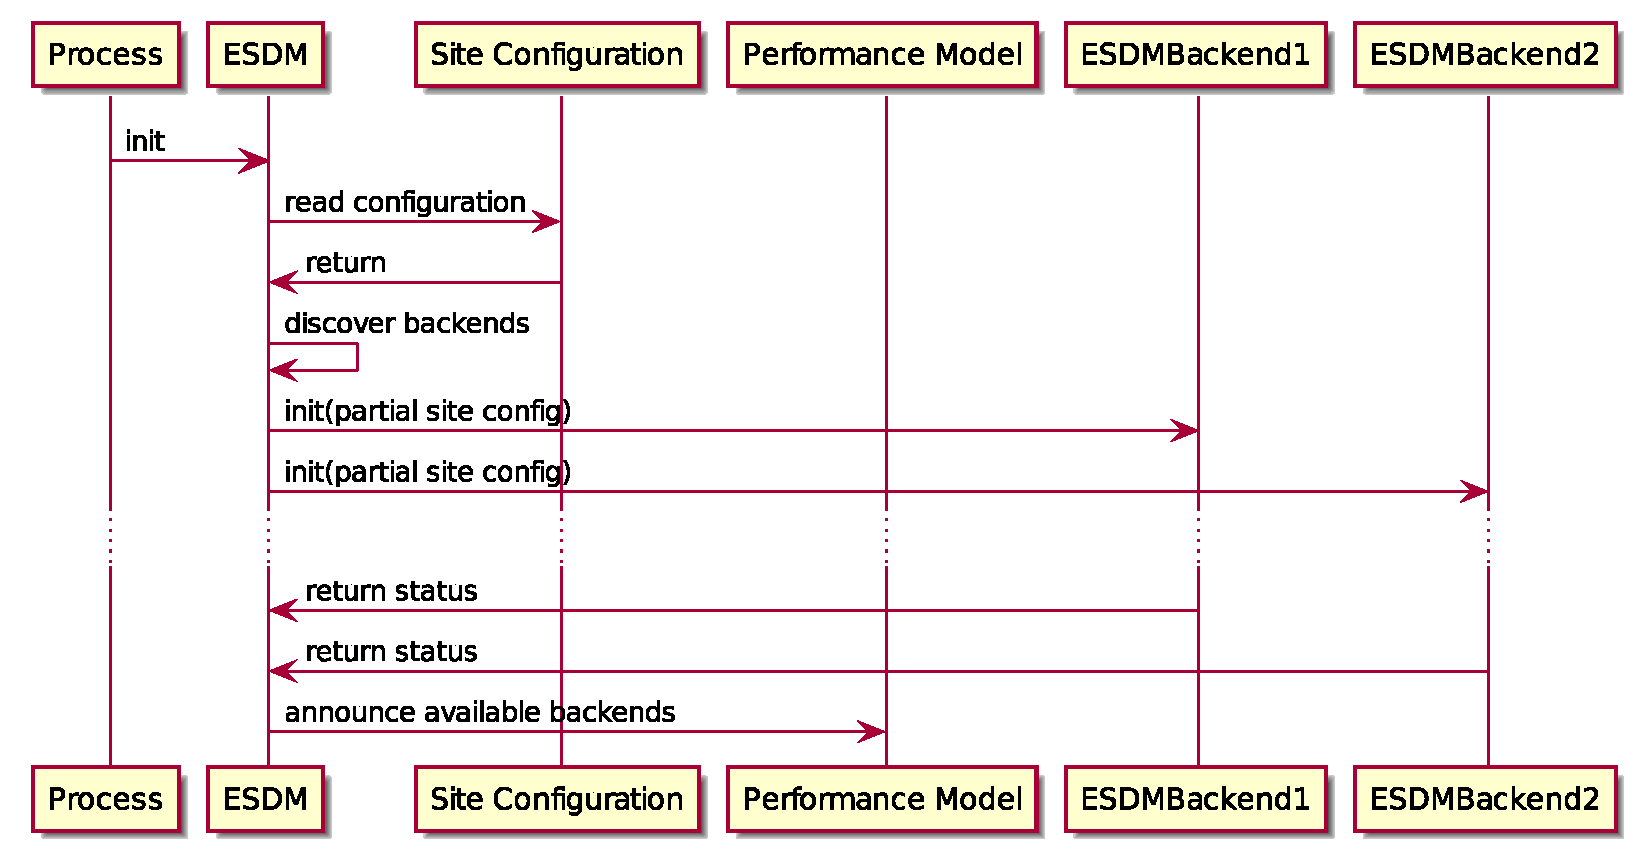
\includegraphics[width=\linewidth]{esdm-components/layout/sequence_init.eps}
	\caption{The initialisation process of the ESDM and the performance model and also the available backends.}
	\label{fig:esdm layout initialisation}
\end{figure}



\subsubsection{Performance Model and Decision Process}
\label{sec: layout/logical/decision}

One approach to find the best backend/backends is to query every backend for a performance estimate and choose the most affordable.
\Cref{fig:esdm layout choose backend} shows in a simplified example how the decision process for a data center with three storage systems may look like.
The decision would gather estimates by calling the performance model (PM) of every backend.
Performance metrics may include:

\begin{itemize}
	\item Latency
	\item Throughput (read/write)
	\item Energy/Cost
	\item Capacity/Fill level
\end{itemize}

Users or administrators may weight which factors are most important for their application.
The decision process has to be configurable because different sites have different requirements.

\begin{figure}
	\centering
	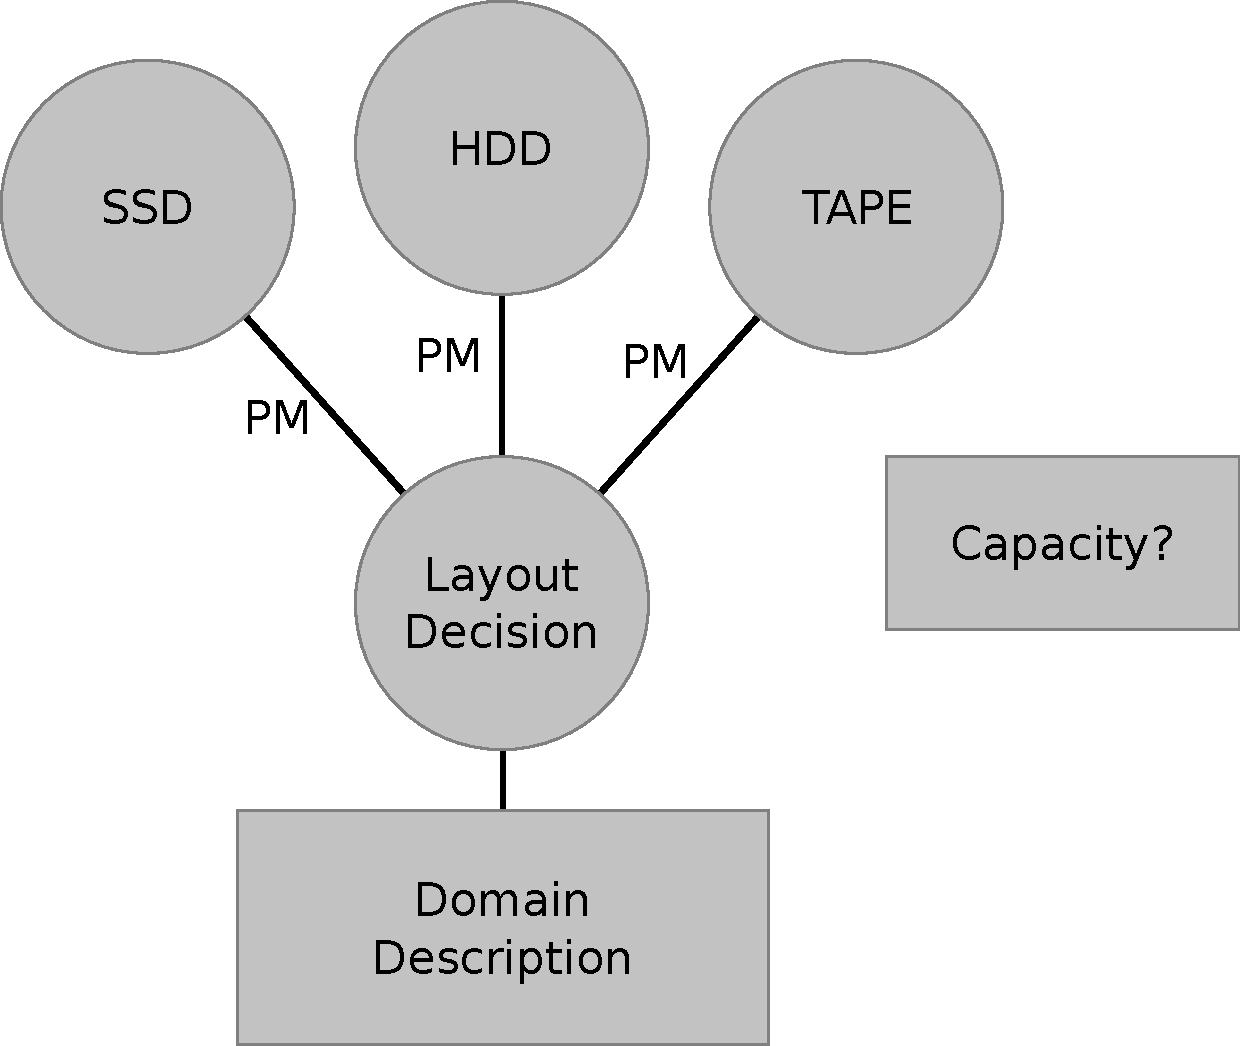
\includegraphics[width=0.5\linewidth]{esdm-components/layout/performance-model.pdf}
	\caption{A layout decision component queries the performance estimates for every backend and also takes the domain into account. Possibly other metrics such as the available capacity for every backend may as well be considered.}
	\label{fig:esdm layout choose backend}
\end{figure}

% Unadressed: When to release allocated memory?


\subsubsection{Layout Reconstruction}

When applications are reading data the ESDM Scheduler consults the layout component for a domain reconstruction.
A subdomain description is passed to the layout component as part of request.
The layout component then requests metadata for the container/variable to be received.
From the list of available fragments the layout component has now to choose a subset of fragments that can be read efficiently from the backends.
To decide which fragments to choose the performance model is consulted.


%%%%%%%%%%%%%%%%%%%%%%%%%%%%%%%%%%%%%%%%%%%%%%
\subsection{Process View}

For the layout component to types of processes can be distinguished:

\begin{itemize}
	\item Layout reconstructions and finding fragmentation
	\item Gathering performance estimates
\end{itemize}

\Cref{fig:esdm layout process view} illustrates the possible process in am UML diagram.
Layout reconstructions may result in multiple requests to multiple ESDM backends.
How ESDM gathers/flushes these fragments concurrently is described in \Cref{component: scheduler}.


\begin{figure}
	\centering
	\includegraphics[width=\linewidth]{esdm-components/layout/process.eps}
	\caption{Multiple process are involved with most applications. For every node the performance decisions maybe different, but in many cases it also maybe desirable to find an estimate collectively. Ultimately the performance estimate needs to be relatively cheap to compute. }
	\label{fig:esdm layout process view}
\end{figure}





%%%%%%%%%%%%%%%%%%%%%%%%%%%%%%%%%%%%%%%%%%%%%%
\subsection{Physical View}

\begin{figure}
	\centering
	\includegraphics[width=\linewidth]{esdm-components/layout/physical.eps}
	\caption{Physical view for the layout component a closely related components.}
	\label{fig:esdm layout  physical view}
\end{figure}

The layout component relies on multiple subcomponents, all of which only exist within the application process.
\Cref{fig:esdm layout physical view} illustrates the distribution and relation of the components across different hardware components.
The site configuration is expected to be pulled from a storage system that can withstand a large number of reading clients.
Nodes may cache the site configuration locally.
The ESDM layout component does require prerequisites from the storage system, but changes to the configuration of the storage system should be reflected in the site configuration.


%%%%%%%%%%%%%%%%%%%%%%%%%%%%%%%%%%%%%%%%%%%%%%%
%\subsection{Development View}
%
%\begin{figure}
%	\centering
%	\includegraphics[width=\linewidth]{esdm-layout/development.eps}
%	\caption{}
%	\label{fig:esdm layout development view}
%\end{figure}




%%%%%%%%%%%%%%%%%%%%%%%%%%%%%%%%%%%%%%%%%%%%%
\clearpage
\section{HDF5+MPI plugin}
\label{frontend: hdf5 + mpi}
This section describes the implications on an existing parallel application that uses one of the supported interfaces such as NetCDF4/HDF5.
The semantics of the API calls will change slightly but typically in a way that is backwards compatible.

\subsection{Logical View}


\begin{figure}
	\centering
	\includegraphics[width=\linewidth]{esdm-hdf5+mpi/logical.eps}
	\caption{Logical view to the HDF+MPI plugin.}
	\label{fig:esdm hdf5 logical view}
\end{figure}

This subsection covers dealing with file names, opening and closing of containers as well as concurrency semantics.
We assume an MPI parallelized application uses HDF5 with MPI support, e.g., parallel HDF5.
The component diagram in \Cref{fig:esdm hdf5 logical view} illustrates how a HDF5/NetCDF ESDM frontend would mediate between the ESDM and an application.
In addition, multiple processes using ESDM can coordinate using MPI, though only ESDM component using MPI is the ESDM HDF5 VOL Plugin.




\subsubsection{Dealing with file names}

Traditionally, when opening a file with NetCDF the filename specifies the location, i.e., a URI where the data resides on a storage system.
We change the notion of the file name to be the descriptor for a virtual container (virtual container descriptor).
The virtual container can be composed of multiple URIs to integrate different variables into one virtual environment on the fly.
Thus, from the reader's perspective it does not matter if data of a model is split into one or multiple physical files; upon read, all those files can be loaded together as if they would already exist in one logical file.
It is also possible to avoid the use of the metadata backend; by specifying the locations of the variables on existing storage media, they can be linked into a virtual container.
One restriction to this approach is the limitation of the length of file names.
To avoid this limitation, we support a prefix to the filename: \texttt{esd-cfg:/} that leads to a simple JSON file that contains the actual definition of the container.

\subsubsection{Open}

Opening a container (as defined by the file name) in ESDM will trigger the master process within the communicator to retrieve the necessary metadata from ESDM and broadcast it to all participating processes.
Since the metadata is serializable to JSON, we can exchange the metadata easily.

\subsubsection{Concurrency semantics}

In general, the system is designed for parallel applications of which processes access data independently of each other.
Still, metadata of internal objects such as containers and variables should be managed and updated explicitly by a single process of the application.
That means, within one parallel (MPI) application, some kind of coordination must take place to allow the shared access to containers, variables and shards.
A correct implementation for this behavior will be performed within the HDF5 VOL plugin.

Data sharing between independent applications is intended to happen after an epoch has been completed.
It is not allowed that multiple parallel applications write data to the same variable at the same time.
This is considered to be sufficient for most scenarios, e.g., a model produces some output; once the epoch  completed, the produced data is post-processed.

\subsubsection{Close}

From the user perspective, closing a file that was opened in write mode, will make the content of the file visible in ESDM and durable for subsequent accesses.
Thus, it updates the metadata, for example, incrementing the epoch of the variables and containers modified and updating the reference counters.

\subsection{Physical View}


\begin{figure}
	\centering
	\includegraphics[width=\linewidth]{esdm-hdf5+mpi/physical.eps}
	\caption{Physical view to the HDF5+MPI plugin.}
	\label{fig:esdm hdf5 physical view}
\end{figure}

ESDM does not change anything of the placement of the processes run by MPI.
\Cref{fig:esdm hdf5 physical view} illustrates the distribution and relation of the components across different hardware components.


\subsection{Process View}

\begin{figure}
	\centering
	\includegraphics[width=\linewidth]{esdm-hdf5+mpi/process.eps}
	\caption{Process view to the HDF5+MPI plugin.}
	\label{fig:esdm hdf5 process view}
\end{figure}

ESDM will start internally threads in the Scheduler component, however, these threads will not call MPI functions or HDF5.
The ESDM plugin in the HDF5 VOL may use MPI functions (or the lightweight library) to coordinate access to central data structures.
\Cref{fig:esdm hdf5 process view} illustrates the process view as far as the HDF5 VOL plugin and MPI coordination is concerned.



%%%%%%%%%%%%%%%%%%%%%%%%%%%%%%%%%%%%%%%%%%%%%
\clearpage
\section{Fuse Legacy + Metadata Mapped Views}
\label{frontend: fuse}

Filesystem in Userspace (FUSE) provides a relatively simple means to export a view to data as a virtual file system, but without the need for special privileges associated with similar techniques. FUSE is thus a popular choice to achieve legacy support for applications that require POSIX-like access semantics.


%%%%%%%%%%%%%%%%%%%%%%%%%%%%%%%%%%%%%%%%%%%%%%
\subsection{Logical View}

\begin{figure}
	\centering
	\includegraphics[width=0.5\linewidth]{esdm-fuse/logical.eps}
	\caption{Based on a FUSE ESDM configuration different views to data are possible. HDF5 files maybe created as soon as a job is known or on the fly.}
	\label{fig:esdm fuse logical view}
\end{figure}

Compatibility to legacy applications is the main motivation to provide a ESDM FUSE  file system.
Allowing different views to the same data based on the available metadata information is another motivation.
Examples for  metadata mappings to a hierarchical namespace could be as follows:

\begin{itemize}
	\item  \texttt{modelname/date/variable.h5}
	\item  \texttt{region/date/modelname/variable.nc}
\end{itemize}

The structure of the hierarchy could be up to the users.
The limit at this point would be the quality of available metadata as it is in already existing metadata catalogues.
\Cref{fig:esdm fuse logical view} illustrates how the ESDM FUSE file system would be used by a scientist.
In an ideal setting, the ESDM has some time to analyse e.g. a submitted job script to figure out which HDF5 will be requested.
The ESDM would then use the HDF5 creator to generate the HDF5 files before the job is started/beginning to read from the file.
After the ESDM HDF5 creator has created the file, the ESDM FUSE would read and write from this file.
If a generated it not used for a while, it may be removed again to make room for more recent requests.


\paragraph{Access Semantics:}
HDF5 files usually allow to be modified to add metadata or update variables and data sets.
The ESDM legacy interface likely will be read only.
A possible update of the original ESDM data structures to reflect changes made to the HDF5 view is not planned, to avoid potential consistency conflicts.
The structure of the HDF5 and the directory structure of available files depends on a ESDM FUSE configuration.



%%%%%%%%%%%%%%%%%%%%%%%%%%%%%%%%%%%%%%%%%%%%%%
\subsection{Development View}
\label{sec: fuse/development}

%
%\begin{figure}
%	\centering
% 	\includegraphics[width=0.5\linewidth]{esdm-fuse/development.eps}
%	\caption{}
%	\label{fig:esdm layout development view}
%\end{figure}


Some applications may not be compatible to HDF5 with virtual object layer (VOL).
For such application it is necessary to export data stored within ESDM as actual HDF5 files.
A FUSE interface allows to automate the export without requiring to generate the actual HDF5 files unless they are requested.
Two approaches for exposing HDF5 files are:

\begin{itemize}
	\item Recreate sections of HDF5/NetCDF files, as they are being read, on the fly. Potentially very complicated, especially for read and write. This is not very desirable from a performance perspective. Refer to \url{https://support.hdfgroup.org/HDF5/doc/H5.format.html} for file format details.
	\item Write a brand new HDF5 file based on the requested data/query.
\end{itemize}

While it maybe in possible to fulfil requests to virtual HDF5 files without generating the actual file, the architecture of HDF5 with different file format drivers leads and HDF5 internal caching makes such an approach unfeasible.


\subsubsection{Use HDF5 to create file on the fly}

The ESDM FUSE interface for HDF5 files should act as a cache layer for HDF5 exports generated on demand, while allowing
to browser available data sets and variables from a file system.
\Cref{fig:fuse hdf5 sequence} illustrates this process in a UML sequence diagram.
A legacy application makes a request to the FUSE file system, which is handled by the ESDM middleware that will use HDF5 to create a HDF5 file.


\begin{figure}
	\centering
	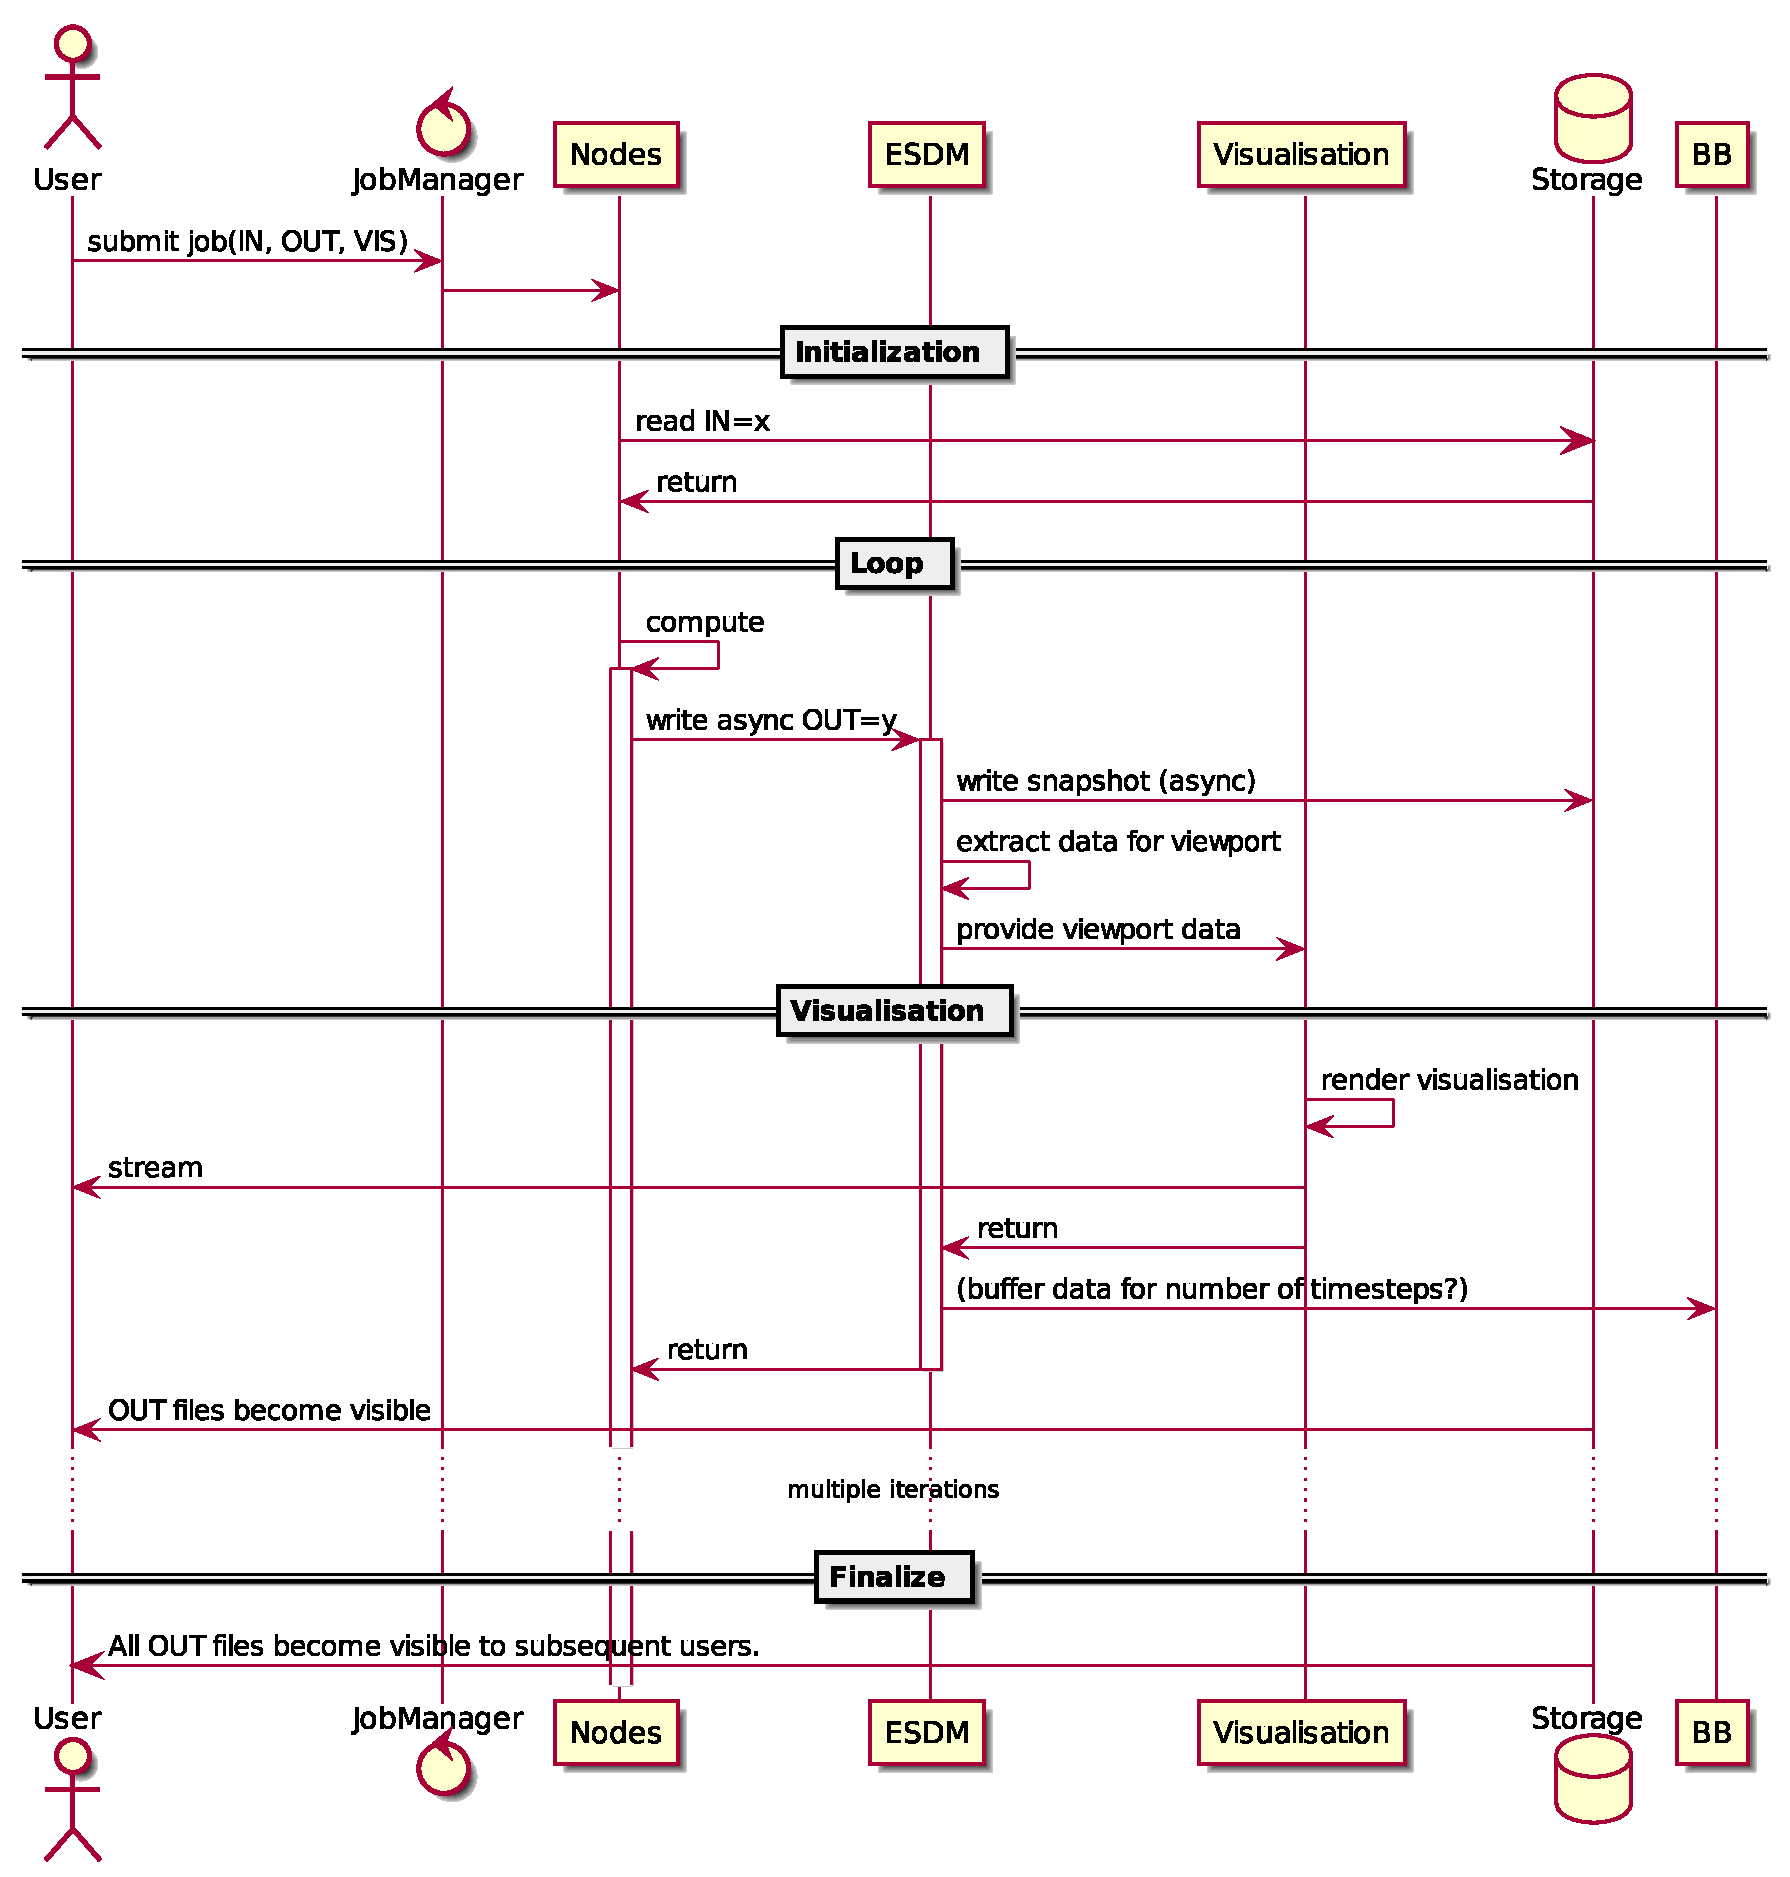
\includegraphics[width=\linewidth]{esdm-fuse/sequence.eps}
	\caption{The simplest approach to expose data to legacy applications by creating actual HDF5 files on the fly and cache them on a file system.}
	\label{fig:fuse hdf5 sequence}
\end{figure}



%%%%%%%%%%%%%%%%%%%%%%%%%%%%%%%%%%%%%%%%%%%%%%
\subsection{Process View}


\begin{figure}
	\centering
	\includegraphics[width=\linewidth]{esdm-fuse/process.eps}
	\caption{Process view to a FUSE legacy backend for ESDM. An application browsers a FUSE file systems which is generated based on the available metadata. As the application opens a file, the ESDM creates a HDF5 file which can be then read just a usual HDF5 file.}
	\label{fig:esdm fuse process view}
\end{figure}

Following the reasoning in \Cref{sec: fuse/development} HDF5 files would need be generated and stored before file access requests can be handled.
\Cref{fig:esdm fuse process view} separates the process of accessing a available file and the actual generation of the file.
If the application is already running and the requests HDF5 file is not already present, the reconstruction can be performed on the node of the application.
If the application is not yet running, the scheduler could start a reconstruction before the application is started.
In both cases a component that generates the HDF5 file is required which is represented by the ESDM HDF5 Creator.







%%%%%%%%%%%%%%%%%%%%%%%%%%%%%%%%%%%%%%%%%%%%%%
\subsection{Physical View}

\begin{figure}
	\centering
	\includegraphics[width=\linewidth]{esdm-fuse/physical.eps}
	\caption{Physical View: Allow legacy applications to access data stored to ESDM by creating HDF5 on the fly or by scanning job files in advance.}
	\label{fig:esdm fuse physical view}
\end{figure}

The provision of a FUSE legacy interface allows for a number different deployment models.
\Cref{fig:esdm fuse physical view} illustrates where the ESDM FUSE related component would be active within the data centre.
To require only little modifications and exploit independent data access FUSE is assumed to be available on the compute nodes.
The scheduler may be modified to start the ESDM HDF5 Creators before spawning a job.
The actual ESDM data as well as temporary HDF5 files would be stored and distributed across multiple storage systems.




%%%%%%%%%%%%%%%%%%%%%%%%%%%%%%%%%%%%%%%%%%%%%
\clearpage
\section{Backend POSIX/Lustre (Using ESDM)}
\label{backend: posix}

Most climate applications today read and write from and to parallel file systems such as Lustre.
The section describes how a POSIX-like backend to the ESDM would handle read and write requests and organise the ESDM data structures.


%%%%%%%%%%%%%%%%%%%%%%%%%%%%%%%%%%%%%%%%%%%%%%
\subsection{Logical View}
\label{backend: posix/logical}

\begin{figure}
	\centering
	\includegraphics[width=\linewidth]{esdm-backends/POSIX/logical.eps}
	\caption{Logical view to the POSIX backend. I/O requests arrive through the ESDM API. The layout component provides a fragmentation (write: site config + perf model / read: as stored in metadata + optimisation candidate). As a result, actual I/O requests are processed by the progress component which calls the backends. The backends and the datatype components work together to convert data according to what is required (read and write differ).}
	\label{fig:backend posix logical view}
\end{figure}

In the previous sections, we have discussed how the scheduler (see \Cref{component: scheduler}) accepts requests by applications and libraries and then consults the layout component (\Cref{component: layout}) to decide on a layout.
In this section, we assume the POSIX backend was chosen.
\Cref{fig:backend posix logical view} illustrates the associated components and which components interact with each other.
Requests made to the POSIX backend can be classified into one of three types.
On the one hand, there are read and write requests to the data.
In addition, there may be metadata lookup, which will in most cases relate to technical metadata.
The following paragraphs explain each of these access types in more detail.


\paragraph{Writing data}
To satisfy write requests, this section extends the use-case description for general writing (see \Cref{uc: independent write}).
The sequence of events relevant to the POSIX backend (also illustrated in \Cref{fig:backend posix sequence write}) unfolds as follows:

\begin{enumerate}
	\item Progress: consults layout about:
	\begin{itemize}
		\item Which Backend?
		\item Which Fragmentation?
	\end{itemize}
	\item Scheduler: processes write calls for all fragments and hands data to POSIX backend
	\item Layout: decides for the specific backend that is suitable for the individual fragment (e.g. row-way serialisation)
	\item Backend: converts between file serialisation and ESDM datatypes
\end{enumerate}

For a POSIX backend, many potential mappings to files and directories are possible.
Which mappings are the most efficient is an open research question and depends on the application.
A straight forward approach is to use the directory structure to map hierarchical concepts, e.g. from NetCDF or HDF5 such as groups and data sets.
The files within the data set directory would include a description of the domain and an additional directory that is used to store the actual fragments.

\begin{figure}
	\centering
	\includegraphics[width=\linewidth]{esdm-backends/POSIX/sequence_write.eps}
	\caption{Sequence Diagram for writes to the POSIX Backend.}
	\label{fig:backend posix sequence write}
\end{figure}



%%%%%%%%%%%%%%%%%%%%%%%%%%%%%%%%%%%%%%%%%%%%%%%%
\paragraph{Reading data}

Analogue to the write case, the reading data with a backend extends the use-case description for general reading (see \Cref{uc: independent read}).
The sequence of events relevant to the POSIX backend (also illustrated in \Cref{fig:backend posix sequence read}) unfolds as follows:

\begin{itemize}
	\item Read arrives
	\item Progress receives requests and splits it potentially into multiple subrequests
	\item Layout loads metadata, consults indexes and collects a sufficient amount of fragments to reconstruct requested (sub)domain in parallel and from the most ``affordable'' backends
	\item Progress (potentially coordinated across multiple processes) issues requests to backends
	\item Backends fetch data and return Fragments
	\item Backend + Layout + Datatype perform necessary conversations
	\item Data is provided to the application
\end{itemize}



\begin{figure}
	\centering
	\includegraphics[width=\linewidth]{esdm-backends/POSIX/sequence_read.eps}
	\caption{Sequence diagram for reads to the POSIX backend.}
	\label{fig:backend posix sequence read}
\end{figure}



\paragraph{Lookup:}

\Cref{sec: viewpoints/logical/data model} introduced the ESDM data model.
A backend is responsible for storing a fragment and finding the fragment again when it is requested.
The POSIX backend will use indexes to allow for a fast search for required fragments.
In addition, fragments are written in sequence from a linked list that allows reconstructing either the domain or the index in case an index is damaged.
Fragments metadata should allow for partial access of fragment.
To allow this a POSIX Fragment wraps the ESDM fragment to attach technical metadata relevant only for the POSIX backend.
A UML diagram illustrating the relationship between POSIX Fragments and ESDM fragments is depicted in \Cref{fig:backend posix fragment}.

\begin{figure}
	\centering
	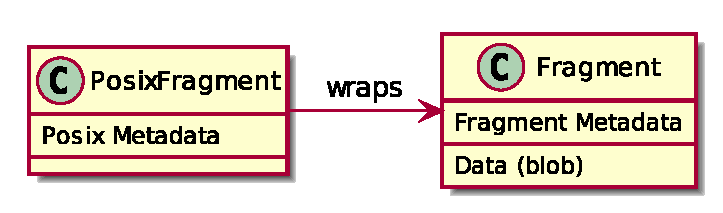
\includegraphics[width=0.5\linewidth]{esdm-backends/POSIX/fragment.eps}
	\caption{The ESDM Fragment features a Metadata section that describes the position within a domain. The actual data is simply a blob. Backends are free to extend ESDM Fragments to their liking.}
	\label{fig:backend posix fragment}
\end{figure}





%%%%%%%%%%%%%%%%%%%%%%%%%%%%%%%%%%%%%%%%%%%%%%
\subsection{Process View}
\label{backend: posix/process}

\begin{figure}
	\centering
	\includegraphics[width=\linewidth]{esdm-backends/POSIX/process.eps}
	\caption{Overview of processes that are necessary or interact/interfere with the POSIX backend.}
	\label{fig:backend posix process view}
\end{figure}

\Cref{fig:backend posix process view} illustrates the process view for the POSIX backend. In addition, interactions between the following services and processes are relevant:


\paragraph{Scheduler component}
The progress component is responsible for handling any sync calls as well as outstanding async calls that have to be passed to the backend.


\paragraph{ESDM Compactor component}
The ESDM compactor may either reorganise POSIX data snippets on their on.. e.g. when running as a daemon that improves and maintains the system health.
As applications issue I/O the progress component may use the ESDM compactor when the decision component determines feasible reorganisation/compactification.


\paragraph{(Competing Load):}
Other resources may access the same storage backend or even the same data.
For example, workflows may compete for access to the same storage target which may influence the decisions used for compactification.


\paragraph{(Service Loads):}
The backends usually employ service workloads that ensure system health.
%How do ESDM and their workloads interfere with each other?




%%%%%%%%%%%%%%%%%%%%%%%%%%%%%%%%%%%%%%%%%%%%%%
\subsection{Physical View}

Active software components related to the ESDM that are involved in handling requests are spread across the application process and when they are finally written on the POSIX storage system as illustrated in \Cref{fig:backend posix physical view}.
No changes to POSIX are assumed, but a POSIX backend will call the interfaces these storage systems expose.

Notice that POSIX in this graphic provides a performance model, which is technically not the case for the current ESDM because the system runtime information such as fill level is not communicated actively by the storage system but are instead collected by, e.g., the ESDM POSIX Backend Plugin.


\begin{figure}
	\centering
	\includegraphics[width=\linewidth]{esdm-backends/POSIX/physical.eps}
	\caption{Physical mapping of components to location of their execution?}
	\label{fig:backend posix physical view}
\end{figure}



%%%%%%%%%%%%%%%%%%%%%%%%%%%%%%%%%%%%%%%%%%%%%%%
%\section{PFS Backend}
%
%\todo{Relocate into Architecture Section?}
%\todo{Probably multiple such use cases to describe the backends.}
%
%Storage entities: files, directories
%
%Permissions:
%* Mapping description
%
%Mapping from containers, variables and fragments:
%A fragment is a file:
%* data
%* support structures (index)
%
%Epoch
%*
%
%
%General description of PFS backend. Motivated by use cases.
%
%



\section{Mongo DB Metadata backend}
\label{backend: mongo}

A prototypical metadata backend will be realised using MongoDB.
Advantages of using MongoDB are that it scales horizontally with the number of servers, provides fault-tolerance and that the document model supports arbitrary schemas.


Each type of object in the data model (container, variable, fragment) becomes a collection with indices on certain fields.
Multikey indices allows indexing array fields such as the references.



\subsection{Logical View}
\label{backend: mongo/logical}

\subsubsection{Metadata}

There are two methods to include metadata, large metadata is includes as a reference to another variable containing the data, small metadata is embedded into the JSON of the MongoDB document.

Besides scientific metadata, the dynamic mapping of data to storage backends requires further metadata that must be managed.
To distinguish technical metadata from scientific metadata, an internal namespace is created.
Relevant technical metadata is shown in \Cref{tbl:additionalTechnicalMetadata} for shards, variables and containers, respectively.

Metadata can be optional (O) or mandatory (M), and either is created automatically or must be set manually via the APIs.
Automatic fields cannot be changed by the user.
Some of the data can be automatically inferred, if not set manually, but manual setting may allow further optimisations.

Some of the metadata is used on several places, for example, information about the data lineage might be used to create several output variables.
In our initial implementation, the metadata is stored redundantly because it
1) simplifies search; 2) enables us to restore data on corrupted storage systems by reading the metadata; 3) reduces contention and potentially false sharing of metadata.
An implementation might decide to reduce this by utilising normalised schemas.

References are the list of objects that are directly used by this object, e.g., other variables that are used to define the data further.

\begin{table}
	\begin{subtable}[t]{\textwidth}
		\begin{tabular}{llll}
			Metadata & Field & Creation & Description\\
			\hline
			Domain   & M & Auto & The subdomain this data covers from the variable\\
			Type     & M & Auto & The (potentially derived) datatype of this shard\\
			Variable & M & Auto & The ID of the varitechnical-on-metadata.texable this data belongs to\\
			Storage  & M & Auto & The storage backend used and its options\\
			References & M & Auto & A list of objects that are referenced by this data\\
			Sealed   & M & Auto & A sealed shard is read-only\\
		\end{tabular}
		\caption{For a shard}
	\end{subtable}

	\begin{subtable}[t]{\textwidth}
		\begin{tabular}{llll}
			Metadata & Field & Creation & Description\\
			\hline
			Domain      & M & Manual & Describes the overall domain\\
			Type   	    & M & Manual & The (potentially derived) datatype\\
			Info   	    & M & Manual & The scientific metadata of this document\\
			References  & M & Auto & A list of objects that are referenced by this data\\
			Permissions & M & Auto/Manual & The owner and permissions \\
			Shards      & M & Auto & The list of shard objects for this variable\\
			Sealed      & M & Auto & A sealed variable is read-only\\
		\end{tabular}
		\caption{For a variable}
	\end{subtable}


	\begin{subtable}[t]{\textwidth}
		\begin{tabular}{llll}
			Metadata & Field & Creation & Description\\
			\hline
			Owner    & O     & Manual   & The owner of this file view (see the permission model)\\
			Info     & O     & Manual   & Additional scientific metadata for this view\\
			Directory & O    & Manual   & Contains a mapping from names to variables\\
			Environment & O  & Automatic & Information about the application run\\
			Permissions & M & Auto/Manual & The owner and permissions \\
			References  & M & Auto & A list of objects that are referenced by this data.
		\end{tabular}
		\caption{For a container}
	\end{subtable}
	\caption{Excerpt of additional technical metadata}
	\label{tbl:additionalTechnicalMetadata}
\end{table}



%\subsection{Metadata mapping: Needs updating}
%\todo{Some examples driven from the use cases}
%

%%%%%%%%%%%%%%%%%%%%%%%%%%%%%%%%%%%%%%%%%%%%%%%%%%%%%%%%%%%%%%%%%%%%%%%%%%%%%%%
\subsubsection{Adaptive Data Mappings}
The typical storage mapping for scientific data format libraries is the file (linear sequence of bytes organized following the POSIX file system representation, i.e. inodes and blocks). Information is translated into a linear array of bytes in the file system using appropriate schemas. Since the data model defined by the data format library can contain complex hierarchies and attributes besides raw data, the final file will contain additional scientific metadata that needs to be accessed using the POSIX-IO data interface (e.g. \texttt{read()} and \texttt{write()}) instead of the file metadata interface (e.g. \texttt{stat()}, \texttt{lookup()}). This makes the storage model adopted by data format libraries incompatible with the typical parallel file system organization, in which metadata and data are splitted apart and assigned to different services for optimal performance. Additionally, new storage system paradigms have emerged in the last years in which files are organized in a flat namespace (e.g. object storage), removing the restrictions imposed by metadata operations like namespace traversal of POSIX file systems. Hierarchical organization can be still achieved using other dedicated storage representations like key-value stores, at the expense of reduced POSIX semantic.

There is therefore a necessity for more flexible data mappings that can take advantage of an increasing number of storage and backend alternatives, improving access efficiency at the same time. There are two different approaches to this problem: the first is to develop a new data mapping schema for every storage backend. This is the solution adopted by the HDF5 library (through the virtual file and the virtual object layers) in which multiple storage backends can be employed by developing a corresponding plugin that contains the right mapping schema. The obvious limitation of this solution is that once the user has selected a certain backend for a file, this cannot be changed without migrating the whole file to another backend. The second approach is more flexible and consists in making the storage backend selection adaptive. This has the advantage of enabling backend storage selection on the fly depending upon the type of data being stored or a set of user/system defined parameters (e.g. list of data placement policies satisfying certain requirements of quality of service).

Our proposed solution is to integrate the adaptive data mappings capabilities just discussed in the layout component of the ESD middleware. The middleware will understand the scientific metadata of other relevant data format libraries and will be able to use multiple storage backends at the same time to store and retrieve different pieces of data. To support multiple formats the datatype component in the ESD middleware will expose a datatype interface similar to the one available in HDF5 (described in Section~\ref{sec: data-formats}). Additionally, the middleware will add significant metadata to be used in the life cycle management and sharing of data. This can include semantic metadata describing which data is needed and how it is going to be used, the required level of resilience, etc. In this context, some metadata can be automatically generated by the middleware or defined by the user and passed to the middleware through an apposite interface (that will be part of the ESD exposed interface).

Legacy codes will have access to data using a familiar POSIX interface exported through an ESD FUSE module. The FUSE module will communicate with the ESD middleware to access data and export it to users using a namespace representation. The mapping schema definition for mapping data between the storage representation and the namespace will be done later in the project.

Another important aspect to consider when talking about adaptive data mappings is the storage tiering, that is, how many levels of storage there are in the system. Historically, HPC applications have relied on parallel file systems as first tier to store and retrieve their data. Besides the parallel file system, most high-end clusters have a second level of archival storage to which data is migrated from the parallel file system using a hierarchical storage manager. Nowadays compute nodes have access to local storage (typically a block device formatted with a local file system) and with the emergence of new storage technologies, such as non-volatile memories, permanent byte addressable memory. The ESD middleware should be able to exploit these local storage resources to implement prefetching strategies (read patterns) and burst buffers (write patterns).

%In the specific case of Mero (Seagate object store system), which represents one of the possible storage backends that has to be supported by the ESD middleware, hierarchical and semantic metadata can be stored in the key-value store service while array data can be stored into objects. In fact, we can think about using more than one object per dataset. This is particularly useful with chunking since every chunk in the dataset can be mapped to a different object, making parallel access to different data units possible without any need for I/O coordination (no false sharing is possible in this case). Of course, I/O coordination still needs to be provided when multiple processes access the same dataset and chunking is not enabled. In this case the ROMIO library already provides a collective I/O implementation that can be reused by the ESD middleware. Whenever needed, false sharing of data can also be avoided by using `persistent file realm' like mechanisms\footnote{This mechanism allows a certain file portion to be assigned to a specific process in the application and makes this assignment persistent across multiple data accesses.}.

%\todo{Giuseppe: you had a very good document on this already can add something here}

%Goal of the dynamic mapping is to create a hierarchical namespace based on the available metadata.
%It is based on the search for objects.
%With the help of FUSE, these mappings can be created based on a user configuration upon mount-time (supports user mounts).
%Inaccessible data, i.e., where the permissions are not sufficient, can be hidden from the namespace.

%An example mapping could be:
%“v.info.model/v.info.environment.date/v.info.experiment.tags/v.info.name <as NC4>”.
%This would show a single NetCDF4 file for each variable.
%If a variable is attached to various tags, then it is shown for each of them.

%“v.info.model/v.info.environment.date/v.domain.time/v.info.name <as NC4>”.
%Would show one file per timestep.

%How to resolve ambiguity?

%Existing containers can also be directly mapped, showing the input and output variables similarly:
%“<c.\_id>/<c.directory>”


%The storage should now how the logical data space maps to physical positions in memory or storage.
%If the storage backends have this knowlege, they can run local operations on the data.

%Alternatives:
%Triangular grid (locally refined), somehow mapped from user-space to a 1D structure which gets mapped to the storage. (Traditional approach)

%Application(data structure) - Mapping - Middleware - Mapping (byte array) - Storage API - Storage backend

%or:

%Application - Middleware - Storage API - Mapping - Storage backend

%Use sth. like MPI datatypes to descripe memory (in the application)
%Add metadata to describe the meaning / semantics, additional gain: resilience because we know which data to replicate to put into triple ECC ...
%Add hints how the data is used / will the used in the future

%Avoid redundant descriptions of memory / storage.
%Users stores a 3D field, it is clear which storage location is responsible for [x,y,z]
%How to store triangles etc.

%Why not store code as description?
%- describes neighborhood?

%Coordinates? Universal coordinates, application coordinates?

%VTK? haben diverse Datenstrukturen hierfÃŒr.


%Separation of concerns...

%Missmatch of Chunks size and application domain

%false sharing

%Pointer Datentyp: strong ptr, weak ptr.
%like Boost usw.


%NVRAM



%%%%%%%%%%%%%%%%%%%%%%%%%%%%%%%%%%%%%%%%%%%%%%%%%%%%%%%%%%%%%%%%%%%%%%%%%%%%%%%
\subsubsection{Technical Metadata}
\label{subsec: technical metadata}

Besides scientific metadata, the dynamic mapping of data to storage backends requires further metadata that must be managed.
To distinguish technical metadata from scientific metadata, an internal namespace is created.
Relevant metadata is shown in \Cref{tbl:additionalTechnicalMetadata} for shards, variables and containers, respectively.

Metadata can be optional (O) or mandatory (M), and either is created automatically or must be set manually via the APIs.
Automatic fields cannot be changed.
Some of the data can be automatically inferred if not set manually, but manual setting may allow further optimizations.

Some of the metadata is used on several places, for example, information about the data lineage might be used to create several output variables.
In our initial implementation, the metadata is stored redundantly as this:
1) simplifies search; 2) enables us to restore data on corrupted storage systems by reading the metadata; 3) reduces contention and potentially false sharing of metadata.
An implementation might decide to reduce this by utilizing a normalized schema.

References is the list of objects that are directly used by this object, e.g., other variables that are used to define the data further.

\begin{table}
\begin{subtable}[t]{\textwidth}
\begin{tabular}{llll}
Metadata & Field & Creation & Description\\
\hline
Domain   & M & Auto & The subdomain this data covers from the variable\\
Type     & M & Auto & The (potentially derived) datatype of this shard\\
Variable & M & Auto & The ID of the variable this data belongs to\\
Storage  & M & Auto & The storage backend used and its options\\
References & M & Auto & A list of objects that are referenced by this data\\
Sealed   & M & Auto & A sealed shard is read-only\\
\end{tabular}
\caption{For a shard}
\end{subtable}

\begin{subtable}[t]{\textwidth}
\begin{tabular}{llll}
Metadata & Field & Creation & Description\\
\hline
Domain      & M & Manual & Describes the overall domain\\
Type   	    & M & Manual & The (potentially derived) datatype\\
Info   	    & M & Manual & The scientific metadata of this document\\
References  & M & Auto & A list of objects that are referenced by this data\\
Permissions & M & Auto/Manual & The owner and permissions \\
Shards      & M & Auto & The list of shard objects for this variable\\
Sealed      & M & Auto & A sealed variable is read-only\\
\end{tabular}
\caption{For a variable}
\end{subtable}

\todo{
	6.X Mero => TODO Seagate
	6.X HDF5+MPI plugin
	* Typical run as MPI+HDF5 application ?
	** Master process, setup files?
	** Beispiel: Workflows using the containers => aus dem Use Case
	"Pipelines/Workflows"
}

\begin{subtable}[t]{\textwidth}
\begin{tabular}{llll}
Metadata & Field & Creation & Description\\
\hline
Owner    & O     & Manual   & The owner of this file view (see the permission model)\\
Info     & O     & Manual   & Additional scientific metadata for this view\\
Directory & O    & Manual   & Contains a mapping from names to variables\\
Environment & O  & Automatic & Information about the application run\\
Permissions & M & Auto/Manual & The owner and permissions \\
References  & M & Auto & A list of objects that are referenced by this data.
\end{tabular}
\caption{For a container}
\end{subtable}
\caption{Excerpt of additional technical metadata}
\label{tbl:additionalTechnicalMetadata}
\end{table}


\paragraph{Example}

This example illustrates data of a predictive model could be stored on the system and the resulting metadata.
The dimensionality of the underlying grid is fixed.

The application uses the following information to drive the simulation:
\begin{itemize}
 \item Timerange: the simulated model time (from a starting datetime to the specified end)
 \item Longitude/Latitude: 1D data field with the coordinates [float]
 \item Temperature: Initial 2D field defined on (lon, lat)
\end{itemize}
A real model would use further parameters to estimate the temperature but these are sufficient to demonstrate the concepts.
This information is either given as parameter to the simulation or read from an input (container).
A mixture of both settings is possible.


The application produces the following output:
\begin{itemize}
  \item Longitude/Latitude: 1D data field with the coordinates [float]
  \item Model time: the current time inside the simulation
  \item Temperature: 2D field defined on (lon, lat, time) [float], containing the precise temperature on the coordinates defined by lon and lat for the given timestep
  \item AvgTemp: 1D field defined on (time) [float]; contains the mean temperature for the given time
\end{itemize}


Upon application startup, we create a new virtual container that provide links to the already existing input.
In \Cref{lst:mongoContainer}, the metadata for the container is shown, after the application is started.
We assume it has used the APIs to provide the information (input, output, scientific metadata).
In this example, we explicitly define the objects used as input; it is possible to also define
the input as an already existing container.
It is also possible to define the input a-priori if the objectIDs are known / looked up prior application run.
The intended output variables could be given with their rough sizes.
This would allow the scheduler to pre-stage the input and ensure that there is enough storage space available for the output.
The environment information is inferred to the info object but can be changed from the user.

\begin{tcbcode}[label={lst:mongoContainer}]{JSON document describing the container}
\begin{lstlisting}
"_id" : ObjectId(".."),
"directory" : {
  "input" : {
    "longitude" : ObjectId(".."),
    "latitude" : ObjectId(".."),
    "temperature" : ObjectId("..")
   },
  "output" {
     "temperature" : ObjectId(".."),
     "avgTemp" : ObjectId("..")
   }
},
"info" : {
  "model" : { "name" : "my model", "version" : "git ...4711" },
  "experiment" : {
    "tags"        : ["simulation", "poisson", "temperature"]
    "description" : "Trivial simulation of temperature using a poisson process"
  },
},
"environment" : {
  "date"  : datetime(2016, 12, 1),
  "system" : "mistral",
  "nodes" : ["m[1-1000]"]
},
"permissions" : {
  "UID"  : 1012,
  "GID"  : 400,
  "group" : "w", # allows read also
  "other" : "r"
},
"references" : {
  [ all links to used object IDs from input / output ]
}
\end{lstlisting}
\end{tcbcode}

The metadata for a single variable is build based on the information available in the container and additional data provided by the user.
An example for the temperature variable is shown in \Cref{lst:mongotemperature}.
When describing the domain that is covered by the variable, there are two alternatives:
1) a reference to an existing variable is embedded and the minimum / maximum value is provided.
This allows to reuse descriptive information as data has to be stored only once. Min and max describe the multidimensional index of the subdomain in the variable that is actually referenced;
2) data becomes embedded into the file. This option is used when the size of the variable is small.

An advantage of option 2) is that searches for data with a certain property do not require to lookup information in additional metadata.

Similarly, information about the data lineage (history) can originally be inferred from the objects linked in the directory mapping.
The metadata of the referenced object must be copied, if the original object is removed.

\begin{tcbcode}[label={lst:mongotemperature}]{JSON document for temperature}
\begin{lstlisting}
"_id" : ObjectId("<TEMPID>"),
"sealed" : true,
"domain" : [
    "longitude" : [ "min" : 0, "max" : 359999, "reference" : ObjectId("..") ],
    "latitude" : [ "min" : 0, "max" : 179999, "reference" : ObjectId("..") ],
    "time" : [ datetime(...), datetime(...), ... ]
  ],
"type" : "float",
"info" : {
  "convention" : "CF-1.0",
  "name" : "temperature",
  "unit" : "K",
  "long description" : "This is the temperature",
  "experiment" : {
    "tags"        : ["simulation", "poisson", "temperature"]
    "description" : "Trivial simulation of temperature using a poisson process"
  },
  "model" : { "name" : "my model", "version" : "git ...4711" },
  "directory" : {
	"input" : {
	  "longitude" : ObjectId("<LONID>"),
	  "latitude" : ObjectId("<LATID>"),
	  "temperature" : ObjectId("<TEMPID>")
	}
  },
  "environment" : {
    "date"    : datetime(2016, 12, 1),
    "system" : "mistral",
    "nodes"  : ["m[1-1000]"]
  },
  "history" : [
  To illustrate the applied mapping, we use a subset of our NetCDF metadata described in \Cref{sec:netcdfDataMapping}.
  The excerpt is given in \Cref{lst:NetCDF-data-map}.
  The mapping of a single logical variable is exemplarily described in


  \begin{tcbcode}[label={lst:NetCDF-data-map}]{NetCDF metadata for one variable}
  \begin{lstlisting}
  dimensions:
  longitude = 480 ;
  latitude = 241 ;
  time = UNLIMITED ; // (1096 currently)
  variables:
  float longitude(longitude) ;
  longitude:units = "degrees_east" ;
  longitude:long_name = "longitude" ;
  float latitude(latitude) ;
  latitude:units = "degrees_north" ;
  latitude:long_name = "latitude" ;
  int time(time) ;
  time:units = "hours since 1900-01-01 00:00:0.0" ;
  time:long_name = "time" ;
  time:calendar = "gregorian" ;
  short sund(time, latitude, longitude) ;
  sund:scale_factor = 0.659209863732776 ;
  sund:add_offset = 21599.6703950681 ;
  sund:_FillValue = -32767s ;
  sund:missing_value = -32767s ;
  sund:units = "s" ;
  sund:long_name = "Sunshine duration" ;

  // global attributes:
  :Conventions = "CF-1.0" ;
  :history = "2015-06-03 08:02:17 GMT by grib_to_netcdf-1.13.1: grib_to_netcdf /data/data04/scratch/netcdf-atls14-a562cefde8a29a7288fa0b8b7f9413f7-lFD4z9.target -o /data/data04/scratch/netcdf-atls14-a562cefde8a29a7288fa0b8b7f9413f7-CyGl1B.nc -utime" ;
  }
  \end{lstlisting}
\end{tcbcode}

To simplify search and identify data clearly, data services such as the WDCC and CERA, that offer data to the community, request scientists to provide additional metadata.
Normally, such data is provided when the results of an experiment is ingested into such a database.
Example metadata is listed in \Cref{tbl:additionalMetadata}.
In existing databases, the listed metadata is split into several fields, e.g. an address and email for persons, for simplicity only a rough overview is given.
Instead of encoding the history as a simple text field, it could
indicate detailed steps including the arguments for the commands and versions and transformations to reproduce the data.
This should include for each step, where and the ti
    #The history for the inputs, if the data lineage must be embedded
    ObjectId(<LONID>) : [
      # Assume LONID does not exist any more
    ],
  ]
},
"permissions" : {
  "UID"  : 1012,
  "GID"  : 400,
  "group" : "w", # allows read also
  "other" : "r"
},
"references" : {
  [ all links to used object IDs ]
},
"shards" : [
  ObjectId(<SHARD1 ID>),
  # For a sealed object, the domains of its shards can optionally be embedded:
  { "reference" : ObjectId(<SHARD2 ID>), "storage" : ... , "domain" },
  ObjectId(<SHARD3 ID>),
  ObjectId(<SHARD4 ID>)
]
\end{lstlisting}
\end{tcbcode}

The variable is split into multiple shards; metadata for one of them is shown in \Cref{lst:mongotemperatureshard}.
Since we assume domain decomposition in the application, the longitude and latitude variables are now only partially stored in a shard.
In the example, we assume two processes create one shard each and the surface of the earth is partitioned into four non-overlapping rectangles.

\begin{tcbcode}[label={lst:mongotemperatureshard}]{JSON document for a shard of the temperature variable}
\begin{lstlisting}
"_id" : ObjectId("<SHARD1 ID>"),
"sealed" : true,
"variable" : ObjectId("<TEMPID>"),
"type" : "float",
"domain" : {
    "longitude" : [ "min" : 0, "max" : 179999, "reference" : ObjectId("..") ],
    "latitude" : [ "min" : 0, "max" : 89999, "reference" : ObjectId("..") ],
    "time" : [ datetime(...), datetime(...), ... ]
  },
"storage" : {
    "plugin" : "pfs",
    "options" : {
      "path" : "/mnt/lustre/testdir/file1",
    },
    "serialization" : "row-major"
  },
"references : [
  ObjectId("<TEMPID>"),
  ObjectId(".."),
  ObjectId("..")
]
\end{lstlisting}
\end{tcbcode}



%%%%%%%%%%%%%%%%%%%%%%%%%%%%%%%%%%%%%%%%%%%%%%%%%%%%%%%%%%%%%%%%%%%%%%%%%%%%%%%
\subsection{Data/Metadata Backend Drivers}
A prototypical metadata backend will be realized using MongoDB.
Advantages of using MongoDB are that it scales horizontally with the number of servers, provides fault-tolerance and that the document model supports arbitrary schemas.



To illustrate the applied mapping, we use a subset of our NetCDF metadata described in \Cref{sec:netcdfDataMapping}.
The excerpt is given in \Cref{lst:NetCDF-data-map}.
The mapping of a single logical variable is exemplarily described in


\begin{tcbcode}[label={lst:NetCDF-data-map}]{NetCDF metadata for one variable}
\begin{lstlisting}
dimensions:
	longitude = 480 ;
	latitude = 241 ;
	time = UNLIMITED ; // (1096 currently)
variables:
	float longitude(longitude) ;
		longitude:units = "degrees_east" ;
		longitude:long_name = "longitude" ;
	float latitude(latitude) ;
		latitude:units = "degrees_north" ;
		latitude:long_name = "latitude" ;
	int time(time) ;
		time:units = "hours since 1900-01-01 00:00:0.0" ;
		time:long_name = "time" ;
		time:calendar = "gregorian" ;
	short sund(time, latitude, longitude) ;
		sund:scale_factor = 0.659209863732776 ;
		sund:add_offset = 21599.6703950681 ;
		sund:_FillValue = -32767s ;
		sund:missing_value = -32767s ;
		sund:units = "s" ;
		sund:long_name = "Sunshine duration" ;

// global attributes:
		:Conventions = "CF-1.0" ;
		:history = "2015-06-03 08:02:17 GMT by grib_to_netcdf-1.13.1: grib_to_netcdf /data/data04/scratch/netcdf-atls14-a562cefde8a29a7288fa0b8b7f9413f7-lFD4z9.target -o /data/data04/scratch/netcdf-atls14-a562cefde8a29a7288fa0b8b7f9413f7-CyGl1B.nc -utime" ;
}
\end{lstlisting}
\end{tcbcode}

To simplify search and identify data clearly, data services such as the WDCC and CERA, that offer data to the community, request scientists to provide additional metadata.
Normally, such data is provided when the results of an experiment is ingested into such a database.
Example metadata is listed in \Cref{tbl:additionalMetadata}.
In existing databases, the listed metadata is split into several fields, e.g. an address and email for persons, for simplicity only a rough overview is given.
Instead of encoding the history as a simple text field, it could
indicate detailed steps including the arguments for the commands and versions and transformations to reproduce the data.
This should include for each step, where and the time when it is performed, and the versions of software used.

It is easily imaginable that most of this information could be useful already when the data is created as it simplifies the search and data management on the online storage.
Some of the data fields become only available after the initial data creation, e.g., the DOI.
Potentially the data must be updated / curated after the data is created.

\begin{table}
\begin{tabular}{ll}
Metadata & Description\\
\hline
Project & The scientific project during which the data is created \\
Institute & The institution which conducted the experiment\\
Person &  A natural person; could be a contact, running the experiment \\
Contact & Reference to person or consortium \\
DOI      & A document object identifier; useful for identifying a data publication\\
Topic     & Some information about the topic of the data / experiment \\
Experiment & Description of this particular experiment \\
History & A list with the history and transformations conducted with the data \\
\end{tabular}
\caption{Excerpt of additional scientific metadata}
\label{tbl:additionalMetadata}
\end{table}












%%%%%%%%%%%%%%%%%%%%%%%%%%%%%%%%%%%%%%%%%%%%%%%%%%%%%%%%%%%%%%%%%%%%%%%%%%%%%%%
\subsection{Mapping of metadata}

To illustrate the applied mapping, we use a subset of our NetCDF metadata described in \Cref{sec:netcdfDataMapping}.
The excerpt is given in \Cref{lst:NetCDF-data-map}.
The mapping of a single logical variable is exemplarily described in \Cref{lst:NetCDF-data-map}.


\begin{tcbcode}[label={lst:NetCDF-data-map}]{NetCDF metadata for one variable}
\begin{lstlisting}
dimensions:
	longitude = 480 ;
	latitude = 241 ;
	time = UNLIMITED ; // (1096 currently)
variables:
	float longitude(longitude) ;
		longitude:units = "degrees_east" ;
		longitude:long_name = "longitude" ;
	float latitude(latitude) ;
		latitude:units = "degrees_north" ;
		latitude:long_name = "latitude" ;
	int time(time) ;
		time:units = "hours since 1900-01-01 00:00:0.0" ;
		time:long_name = "time" ;
		time:calendar = "Gregorian" ;
	short sund(time, latitude, longitude) ;
		sund:scale_factor = 0.659209863732776 ;
		sund:add_offset = 21599.6703950681 ;
		sund:_FillValue = -32767s ;
		sund:missing_value = -32767s ;
		sund:units = "s" ;
		sund:long_name = "Sunshine duration" ;

// global attributes:
		:Conventions = "CF-1.0" ;
		:history = "2015-06-03 08:02:17 GMT by grib_to_netcdf-1.13.1: grib_to_netcdf /data/data04/scratch/netcdf-atls14-a562cefde8a29a7288fa0b8b7f9413f7-lFD4z9.target -o /data/data04/scratch/netcdf-atls14-a562cefde8a29a7288fa0b8b7f9413f7-CyGl1B.nc -utime" ;
}
\end{lstlisting}
\end{tcbcode}

To simplify search and identify data clearly, data services such as the WDCC and CERA, that offer data to the community, request scientists to provide additional metadata.
Normally, such data is provided when the results of an experiment is ingested into such a database.
Example metadata is listed in \Cref{tbl:additionalMetadata}.
In existing databases, the listed metadata is split into several fields, e.g. an address and email for persons, for simplicity only a rough overview is given.
Instead of encoding the history as a simple text field, it could
indicate detailed steps including the arguments for the commands and versions and transformations to reproduce the data.
This should include for each step, where and the time when it is performed, and the versions of software used.

It is easily imaginable that most of this information could be useful already when the data is created as it simplifies the search and data management on the online storage.
Some of the data fields become only available after the initial data creation, e.g., the DOI.
Potentially the data must be updated / curated after the data is created.

\begin{table}
\begin{tabular}{ll}
Metadata & Description\\
\hline
Project & The scientific project during which the data is created \\
Institute & The institution which conducted the experiment\\
Person &  A natural person; could be a contact, running the experiment \\
Contact & Reference to person or consortium \\
DOI      & A document object identifier; useful for identifying a data publication\\
Topic     & Some information about the topic of the data / experiment \\
Experiment & Description of this particular experiment \\
History & A list with the history and transformations conducted with the data \\
\end{tabular}
\caption{Excerpt of additional scientific metadata}
\label{tbl:additionalMetadata}
\end{table}



\subsection{Example}

This example illustrates data of a predictive model could be stored on the system and the resulting metadata.
The dimensionality of the underlying grid is fixed.

The application uses the following information to drive the simulation:
\begin{itemize}
	\item Time Range: the simulated model time (from a starting datetime to the specified end)
	\item Longitude/Latitude: 1D data field with the coordinates [float]
	\item Temperature: Initial 2D field defined on (lon, lat)
\end{itemize}
A real model would use further parameters to estimate the temperature but these are sufficient to demonstrate the concepts.
This information is either given as parameter to the simulation or read from an input (container).
A mixture of both settings is possible.


The application produces the following output:
\begin{itemize}
	\item Longitude/Latitude: 1D data field with the coordinates [float]
	\item Model time: the current datatime for the simulation
	\item Temperature: 2D field defined on (lon, lat, time) [float], containing the precise temperature on the coordinates defined by lon and lat for the given timestep
	\item AvgTemp: 1D field defined on (time) [float]; contains the mean temperature for the given time
\end{itemize}

\subsubsection{Container}

Upon application startup, we create a new virtual container that provide links to the already existing input.
In \Cref{lst:mongoContainer}, the metadata for the container is shown, after the application is started.
We assume it has used the APIs to provide the information (input, output, scientific metadata).
In this example, we explicitly define the objects used as input; it is possible to also define
the input as an already existing container.
It is also possible to define the input a priori if the object IDs are known / looked up prior application run.
The intended output variables could be given with their rough sizes.
This would allow the scheduler to pre-stage the input and ensure that there is enough storage space available for the output.
The environment information is inferred to the info object but can be changed from the user.

\begin{tcbcode}[label={lst:mongoContainer}]{JSON document describing the container}
	\begin{lstlisting}
	"_id" : ObjectId(".."),
	"directory" : {
		"input" : {
			"longitude" : ObjectId(".."),
			"latitude" : ObjectId(".."),
			"temperature" : ObjectId("..")
		},
		"output" {
			"temperature" : ObjectId(".."),
			"avgTemp" : ObjectId("..")
		}
	},
	"info" : { # This is the scientific metadata
		"model" : { "name" : "my model", "version" : "git ...4711" },
		"experiment" : {
			"tags"        : ["simulation", "Poisson", "temperature"]
			"description" : "Trivial simulation of temperature using a Poisson process"
		},
	},
	"environment" : {
		"date"  : datetime(2016, 12, 1),
		"system" : "mistral",
		"nodes" : ["m[1-1000]"]
	},
	"permissions" : {
		"UID"  : 1012,
		"GID"  : 400,
		"group" : "w", # allows read also
		"other" : "r"
	},
	"references" : {
		[ all links to used object IDs from input / output ]
	}
	\end{lstlisting}
\end{tcbcode}

\subsubsection{Variable}

The metadata for a single variable is build based on the information available in the container (such as permissions) and additional data provided by the user.
Indeed, part of the metadata is replicated between container and variable as this preserves information about the creation of the variable that will typically not change during the lifetime of the variable.

An example for the temperature variable is shown in \Cref{lst:mongotemperature}.
When describing the domain that is covered by the variable, there are three alternatives:
1) a reference to an existing variable is embedded and the minimum / maximum value is provided.
This allows reusing descriptive information as data has to be stored only once. Min and max describe the multidimensional index of the subdomain in the variable that is actually referenced;
2) data becomes embedded into the file. This option is used when the size of the variable is small.
An advantage of option 2) is that searches for data with a certain property do not require to lookup information in additional metadata.

Similarly, information about the data lineage (history) can originally be inferred from the objects linked in the directory mapping.
In that case, the metadata of the referenced object must be copied, if the original object is removed.

3) A plugin for the interpretation and mapping of the coordinate system is used.
The plugin name must be stored and the respective parameters to identify the coordinates stored.


\begin{tcbcode}[label={lst:mongotemperature}]{JSON document for temperature}
	\begin{lstlisting}
	"_id" : ObjectId("<TEMPID>"),
	"sealed" : true,
	"domain" : [
		"longitude" : [ "min" : 0, "max" : 359999, "reference" : ObjectId("..") ],
		"latitude" : [ "min" : 0, "max" : 179999, "reference" : ObjectId("..") ],
		"time" : [ datetime(...), datetime(...), ... ]
	],
	"type" : "float",
	"info" : {
		"convention" : "CF-1.0",
		"name" : "temperature",
		"unit" : "K",
		"long description" : "This is the temperature",
		"experiment" : {
			"tags"        : ["simulation", "Poisson", "temperature"]
			"description" : "Trivial simulation of temperature using a Poisson process"
		},
		"model" : { "name" : "my model", "version" : "git ...4711" },
		"directory" : {
			"input" : {
				"longitude" : ObjectId("<LONID>"),
				"latitude" : ObjectId("<LATID>"),
				"temperature" : ObjectId("<TEMPID>")
			}
	},
	"environment" : {
		"date"    : datetime(2016, 12, 1),
		"system" : "mistral",
		"nodes"  : ["m[1-1000]"]
	},
	"history" : [
		...
	],

	"permissions" : {
		"UID"  : 1012,
		"GID"  : 400,
		"group" : "w", # allows read also
		"other" : "r"
	},
	"references" : {
		[ all links to used object IDs ]
	},
	"shards" : [
		ObjectId(<SHARD1 ID>),
		# For a sealed object, the domains of its shards can optionally be embedded:
		{ "reference" : ObjectId(<SHARD2 ID>), "storage" : ... , "domain" },
		ObjectId(<SHARD3 ID>),
		ObjectId(<SHARD4 ID>)
	]
	\end{lstlisting}
\end{tcbcode}

\subsubsection{Shards}

The variable is split into multiple shards; metadata for one of them is shown in \Cref{lst:mongotemperatureshard}.
Since we assume domain decomposition in the application, the longitude and latitude variables are now only partially stored in a shard.
In the example, we assume two processes create one shard each and the surface of the earth is partitioned into four non-overlapping rectangles.

\begin{tcbcode}[label={lst:mongotemperatureshard}]{JSON document for a shard of the temperature variable}
\begin{lstlisting}
"_id" : ObjectId("<SHARD1 ID>"),
"sealed" : true,
"variable" : ObjectId("<TEMPID>"),
"type" : "float",
"domain" : {
	"longitude" : [ "min" : 0, "max" : 179999, "reference" : ObjectId("..") ],
	"latitude" : [ "min" : 0, "max" : 89999, "reference" : ObjectId("..") ],
	"time" : [ datetime(...), datetime(...), ... ]
},
"storage" : {
	"plugin" : "pfs",
	"options" : {
		"path" : "/mnt/lustre/testdir/file1",
	},
	"serialisation" : "row-major"
},
"references : [
	ObjectId("<TEMPID>"),
	ObjectId(".."),
	ObjectId("..")
]
\end{lstlisting}
\end{tcbcode}


\subsection{Physical View}
\label{backend: mongo/physical}

The MongoDB servers will be deployed on the HPC cluster.
Due to the scalability of the infrastructure, the number of servers can be adjusted to the experienced load.


\subsection{Process View}
\label{backend: mongo/process}

We are using the typical deployment of MongoDB including all the services it provides such as the mongo daemon.

% \subsection{Development View}
% \label{backend: mongo/development}




%%%%%%%%%%%%%%%%%%%%%%%%%%%%%%%%%%%%%%%%%%%%%
\clearpage
\section{Mero Backend}
\label{backend: mero}

%%%%%%%%%%%%%%%%%%%%%%%%%%%%%%%%%%%%%%%%%%%%%%
\subsection{Logical View}

Mero is an Exascale ready Object Store system developed by Seagate and built to remove the performance limitations typically found in
other designs. Unlike similar storage systems (e.g., Ceph and DAOS) Mero does
not rely on any other file system or raid software to work. Instead, Mero can
directly access raw block storage devices and provide consistency, durability
and availability of data through dedicated core components. \\

Clovis is the user-space interface exported by Mero for use by the Mero
applications.
Examples of Mero applications are: Mero file system client (m0t1fs), Lustre HSM backend (part of Castor-A200).
ESD middleware will also uses Clovis interfaces to access and manage Mero system.
The logical view for interactions between ESDM and Clovis/Mero is illustrated in \Cref{fig:mero backend logical view}.
 \\
As an object storage, Mero has two types of "objects". In Mero, they are called
Entities, while in object storage, they might be called objects. These
two types of entities are: \\
object, is an array of fixed-size blocks, \\
index, is a key-value store. An index stores records, each record consisting of
       a key and a value. Keys and values within the same index can be of variable
       size. Keys are ordered by the lexicographic ordering of their bit-level
       representation. Records are ordered by the key ordering. Keys are unique
       within an index.\\

Mero defined a set of operations for every type of entities. Mero realm is a
spatial and temporal part of system with a prescribed access discipline.
Objects, indices and operations live in realm. An entity exists in some realm
and has a 128-bit identifier, unique within a Mero cluster and never re-used.
Identifier management is up to the application, except that some identifiers
are reserved for system usage. \\
Generic operations for all entities are: create and delete. They are used to
create a new entity and delete an existing entity. Object has the following
specific operations:
\\
\begin{longtable}{|>{\centering\arraybackslash} m{5.5cm} | >{\centering\arraybackslash} m{6cm} |}\hline\hline
        \cellHeader Mero Object Operation & \cellHeader Description \\ \hline
	READ  & transfer blocks and block attributes from an object to application buffers; \\ \hline
	WRITE & transfer blocks and block attributes from application buffers to an object; \\ \hline
	ALLOC & pre-allocate certain blocks in an implementation-dependent %
                manner. This operation guarantees that consecutive WRITE onto %
                pre-allocated blocks will not fail due to lack of storage space;            \\ \hline
	FREE  & free storage resources used by specified object %
                blocks. Consecutive reads from the blocks will return zeroes.               \\ \hline
        \caption{Mero Object Operations}
\end{longtable}

Index has the following specific operations:
\\
\begin{longtable}{|>{\centering\arraybackslash} m{5.5cm} | >{\centering\arraybackslash} m{6cm} |}\hline\hline
        \cellHeader Mero Index Operation & \cellHeader Description \\ \hline

	GET  &  given a set of keys, return the matching records from the index;    \\ \hline
	PUT  &  given a set of records, place them in the index, overwriting %
	        existing records if necessary, inserting new records otherwise;     \\ \hline
	DEL  &  given a set of keys, delete the matching records from the index;    \\ \hline
	NEXT &  given a set of keys, return the records with the next (in the %
                ascending key order) keys from the index.                           \\ \hline
	LOOKUP  &  given a key, check existence of a record;                        \\ \hline
        \caption{Mero Index Operations}
\end{longtable}



ESD middleware can use Mero indices to store small data and metadata, and objects
to store raw data. For example, Mero indices can be used to keep track of
containers, corresponding variables and shard inside them. Each container will
be represented as an index in Mero. The metadata of this container, the metadata
of all the contained variables, shards and chunks, is stored as key-value records
in this index. Data of variables, shards and chunks can be stored as different
Mero objects. \\

HDF5 file stored in a POSIX file system is identified by its full path name.
ESD middleware needs to keep the mapping from a HDF5 file to Mero identifier of
the index. From this index, ESD middleware can get all metadata for associated
containers and variables and other information. ESD middleware may store the
mapping from HDF5 identity to Mero index identifier in external configuration
storage, e.g. MongoDB, RDBMS, or POSIX file system. Nevertheless, ESD middleware
can also store this mapping in Mero index, too. This index will be a pre-defined
index, with well-known identifier. ESD middleware can initialize this index
at the first of system deployment, and consult it later for this mapping.

\begin{figure}
	\centering
	\includegraphics[width=\linewidth]{esdm-backends/mero/logical.eps}
	\caption{Logical view to the Mero backend. I/O requests arrive through the ESDM API. The layout component provides metadata. As a result actual I/O requests are processed by the progress component which calls the backends. The backends and the datatype components work together to convert data according to what is required (again and read and write differ).}
	\label{fig:mero backend logical view}
\end{figure}


\paragraph{Writing data}


The following sequence extends the Use-Case description for general writing
(see \Cref{uc: independent write}).
A sequence diagram for the chain of events is provided by \Cref{fig:mero backend sequence write}.

\begin{itemize}
	\item Progress: consult layout about:
	\begin{itemize}
		\item the identifier(s) of Mero indices to store or update metadata.
		\item the identifier(s) or Mero objects to store or update raw data. %
		      If this is a write to non-exist container, identifiers are generated
		      according to Mero rules.
	\end{itemize}
	\item Progress: if Mero indices/objects don't exist, create them with proper attributes
	\item Progress: GET some records from index if necessary to update some metadata, %
			and prepare metadata to write
	\item Progress: READ blocks from objects if write request is not block-aligned, %
			i.e. partial write. Prepare the in-memory buffer for destination blocks.
	\item Progress: WRITE buffers into blocks of corresponding objects with Mero %
			Clovis object WRITE interface.
	\item Progress: PUT key-value records to index with Mero Clovis index interface.
	\item Progress: Update layout information if necessary
	\item Progress: Wait on Mero back-end until metadata and data are stable on Mero back-end.
	\item Progress: return to upper layer from ESD middleware
\end{itemize}

\begin{figure}
	\centering
	\includegraphics[width=\linewidth]{esdm-backends/mero/sequence_write.eps}
	\caption{Mero backend sequence write}
	\label{fig:mero backend sequence write}
\end{figure}


\paragraph{Reading data}

The following sequence extends the Use-Case description for general reading
(see \Cref{uc: independent read}).
A sequence diagram for the chain of events is provided by \Cref{fig:mero backend sequence read}.

\begin{itemize}
	\item Progress: consult layout about:
	\begin{itemize}
		\item the identifier(s) of Mero indices to store or update metadata.
		\item the identifier(s) or Mero objects to store or update raw data.
	\end{itemize}
	\item Progress: GET necessary key-value records from Mero index and parse the %
			metadata to get information needed by reading.
	\item Progress: With the metadata, layout, mapping the target read to proper object
			and offset blocks.
	\item Progress: READ target blocks from objects, and fill in user buffers.
	\item Progress: return data to upper layer from ESD middleware
\end{itemize}
\begin{figure}
	\centering
	\includegraphics[width=\linewidth]{esdm-backends/mero/sequence_read.eps}
	\caption{Mero backend sequence read}
	\label{fig:mero backend sequence read}
\end{figure}



\paragraph{Lookup:}

The following algorithms are used to store metadata and the steps used to
find out the Mero object blocks mapped to fragments.

On a POSIX file system, a HDF5 file is identified by its full path. On a Mero
back-end, ESD middleware needs to keep the mapping from HDF5 identity to Mero
index identifier. This is a 128-bit integer. All the metadata of this HDF5 are
stored in this Mero index as key-value records. They are: \\
\begin{longtable}{|>{\centering\arraybackslash} m{5.5cm} | >{\centering\arraybackslash} m{6cm} |}\hline\hline
        \cellHeader key & \cellHeader value \\ \hline
	Name           &  String: the name (i.e. identifier)                      \\ \hline
	"ATTR" + Path  &  The attribute of the path. The path is the format of %
			  "/group1/group2/variable\_1". The attribute may be %
			  encoded in some format, e.g. JSON or something. This will %
			  be defined in detailed design.                          \\ \hline
	"OBJ" + Path   &  list of 128-bit identifier of Mero objects %
			  if the variable is stored in a single object, %
			  this would be the only identifier. If the variable %
			  is partitioned into several shards, this would be a list of
			  identifier of Mero object. The shard size and other metadata %
			  would be stored in the above attribute.                  \\ \hline
	Datatype Name  &  Datatype definition in binary mode or string. %
			  This is the named datatype shared by multiple variable.  \\ \hline
	   ...         &   ...                                                     \\ \hline
        \caption{Metadata Schema}
\end{longtable}

The lookup process is to GET all records from Mero index, and parse them to
reconstruct the in-memory metadata.

%%%%%%%%%%%%%%%%%%%%%%%%%%%%%%%%%%%%%%%%%%%%%%
\subsection{Process View}


ESD middleware will use Clovis interfaces to manage and access a Mero cluster.
\Cref{fig:mero backend process view} illustrates the processes and services related to the Mero backend.


\begin{figure}
	\centering
	\includegraphics[width=\linewidth]{esdm-backends/mero/process.eps}
	\caption{Overview of processes that are necessary or interact/interfere with the Mero backend.}
	\label{fig:mero backend process view}
\end{figure}

\paragraph{Progress component:}
The progress component is responsible for handling any sync calls as well as
outstanding asynchronous calls that have to be passed to the backend. All Mero Clovis
operations are asynchronous (except for the wait() operations).

\paragraph{Clovis Instance component:}
Clovis instance is a collection of in-memory data structures and their state machines.
ESD middleware keeps a handle to this instance. All communications with Mero
is through this instance. Internally, Clovis uses Mero protocols to communicate with
various Mero services.

\paragraph{Service Management component:}
Mero provides the Clovis interface to manage and access its objects and indices.
Mero also provide a serial of utilities to manage and configure its cluster,
monitor various services, poll system events, and trigger specific operations.
ESD middleware can leverage these interfaces and utilities to communicate with
Mero cluster, and manage all kinds of services and configuration.
\\
The main services
that an application (here is ESD middleware) needs to communicate are:
MeroConfd (configuration and management), MeroRMS (transaction), MeroIOS (index
and object operations).


%%%%%%%%%%%%%%%%%%%%%%%%%%%%%%%%%%%%%%%%%%%%%%
\subsection{Development View}

ESD middleware will use Clovis interfaces to manage and access a Mero cluster.
\Cref{fig:mero backend development view} illustrates the development view of the Mero backend.
ESD middleware code needs to link with Mero Clovis library to access Mero cluster.
Clovis provides interfaces in the C language, currently. All Clovis index and object
operations are asynchronous (except for the wait() operation). A Clovis transaction
is a collection of operations atomic in the face of failures.

\begin{figure}
	\centering
	\includegraphics[width=0.25\linewidth]{esdm-backends/mero/development.eps}
	\caption{Development View of Mero backend}
	\label{fig:mero backend development view}
\end{figure}


%%%%%%%%%%%%%%%%%%%%%%%%%%%%%%%%%%%%%%%%%%%%%%
\subsection{Physical View}

Mero storage cluster is relatively an independent system in this case. It can be
managed by Mero utilities. It can also be serving other applications at the
same time. That means, ESD middleware can be one of the applications using
this Mero deployment.
\Cref{fig:backend mero physical view} illustrates the physical view for the Mero backend.

Mero cluster can be configured with different redundant parameters for its
entities. Pool width, [data units, parity units, spare units] for parity
groups of an entity, etc. are those parameters to determine the data redundancy
model, data utilization, performance, and availability. Different configurations
have different mappings from logical data to its physical locations on disks.
But ESD middleware don't have to care about this mapping. ESD middleware uses
Clovis to manage and access Mero entities (Mero indices and objects).
If needed, ESD middleware can use Clovis to create entities with different redundant parameters than the system defaults.

\begin{figure}
	\centering
	\includegraphics[width=\linewidth]{esdm-backends/mero/physical.eps}
	\caption{Physical mapping of components to location of their execution}
	\label{fig:backend mero physical view}
\end{figure}



%%%%%%%%%%%%%%%%%%%%%%%%%%%%%%%%%%%%%%%%%%%%%
\clearpage
\section{WOS Backend}
\label{backend: wos}

%%%%%%%%%%%%%%%%%%%%%%%%%%%%%%%%%%%%%%%%%%%%%%
This section describes the features of the WOS Backend and how it interacts with the different ESDM components in order to perform the read and write activity on behalf of the user applications.

\subsection{Logical View}

The DDN WOS object storage solution (see \Cref{WOS background}) represents a storage system architecture which manages data as objects, automatically storing files in the cloud in a geographically agnostic manner. Each object is stored with a unique OID that is used to retrieve the related data, delete them of verify the existence.
The logical view for interactions between ESDM and Clovis/Mero is illustrated in \Cref{fig:WOS backend logical view}.

To interact with the WOS cluster, DDN provides API for C++, JAVA and Python languages and an HTTP Restful interface; in particular operations as Put, Get, Delete, Exists, Reserve and PutOID are allowed in blocking and non-blocking form.

\begin{figure}
	\centering
	\includegraphics[width=\linewidth]{esdm-backends/WOS/logical.eps}
	\caption{Logical view to the WOS backend. I/O requests arrive through the ESDM API. The layout component provides a fragmentation based on site configuration and performance model. As a result actual I/O requests are processed by the progress component which calls the backends providing the needed metadata. The backends and the datatype components work together to convert data according to what is required.}
	\label{fig:WOS backend logical view}
\end{figure}

\paragraph{Writing data:}
The following sequence extends the Use-Case description for general writing (see \Cref{uc: independent write}).
A sequence diagram for the chain of events is provided by \Cref{fig:WOS backend sequence write}.

\begin{itemize}
	\item Progress consults layout about the choice of the most suitable backend and the proper fragmentation.
	\item Progress sends data to WOS backend.
	\item WOS backend accepts the incoming data properly managing the correct datatype conversion.
	\item WOS backend creates a new WOS Object.
	\item WOS Storage returns the corresponding Object Identifier (OID)
	\item WOS backend saves data to the WOS Storage
	\item WOS backend returns the OID to the Progress module
\end{itemize}

\begin{figure}
	\centering
	\includegraphics[width=\linewidth]{esdm-backends/WOS/sequence_write.eps}
	\caption{WOS backend sequence write}
	\label{fig:WOS backend sequence write}
\end{figure}

\paragraph{Reading data:}
The following sequence extends the Use-Case description for general reading (see \Cref{uc: independent read}).
A sequence diagram for the chain of events is provided by \Cref{fig:WOS backend sequence read}.

\begin{itemize}
	\item Progress and Layout work together in order to eventually split the request into multiple sub requests, one for each fragment to retrieve
	\item Layout collects the needed metadata related to the fragments to retrieve
	\item Progress forward the request to the WOS backend; multiple requests could be sent in parallel
	\item WOS backend retrieves data from the WOS Storage based on OID (Object Identifier)
	\item WOS backend performs the needed datatype conversion
	\item WOS Backend returns data
	\item Data is provided to application
\end{itemize}

It is worth noting that WOS storage manages data in binary format only: no information about data type need to be passed to the storage for writing or reading. The WOS backend, the Layout and the Datatype performs the needed communications for properly managing the different datatypes.

\begin{figure}
	\centering
	\includegraphics[width=\linewidth]{esdm-backends/WOS/sequence_read.eps}
	\caption{WOS backend sequence read}
	\label{fig:WOS backend sequence read}
\end{figure}

\paragraph{Lookup:}
WOS Objects relies on the concept of Object Identifier: each Object is associated to a unique OID and once used an OID cannot be reassigned. OID is the identifier needed by the application for accessing the object and retrieving its data. As stated before, objects are saved into the storage in binary format (for instance mapped as a pointer to a \textit{void} variable in C++ code): user applications need to provide the proper mapping to the final datatype.

Fragments are associated to WOS Objects: the lookup phase is allowed by using the correct OID stored in the metadata backend and provided to the WOS backend to perform the association with the related object. 


%%%%%%%%%%%%%%%%%%%%%%%%%%%%%%%%%%%%%%%%%%%%%%
\subsection{Process View}

\textbf{Progress Component} The progress component is responsible to manage the interactions with the WOS backend, in terms of synchronous and asynchronous call handling. It communicates with the ESDM\textunderscore WOS\textunderscore Service exchanging the proper information about data transferring, metadata management and status of the processes.
\Cref{fig:WOS backend process view} illustrates the processes and services related to the WOS backend.

\textbf{ESDM\textunderscore WOS\textunderscore Service} The ESDM\textunderscore WOS\textunderscore Service represents the middleware between the progress component and the WOS System Storage. It accepts requests incoming from the progress component concerning data and/or metadata management, fragments read and write. The ESDM\textunderscore WOS\textunderscore Service is able to translate such requests into WOS Cluster call which finalizes the operations to the WOS Storage. As supported by the WOS architecture, the ESDM\textunderscore WOS\textunderscore Service is able to manage blocking and non-blocking calls on behalf of the progress component.\\

\textbf{WOS Cluster} The WOS Cluster represents the remote host pool and services able to accept, manage and finalize the incoming requests/data from the ESDM\textunderscore WOS\textunderscore Service. It hosts the WOS Storage and physically handles the retrieval of the requested information triggered by the higher level applications and services.

\begin{figure}
	\centering
	\includegraphics[width=\linewidth]{esdm-backends/WOS/process.eps}
	\caption{Overview of processes and entities involved in the interaction with the WOS backend}
	\label{fig:WOS backend process view}
\end{figure}


%%%%%%%%%%%%%%%%%%%%%%%%%%%%%%%%%%%%%%%%%%%%%%
\subsection{Development View}

The interactions between the ESD middleware and the WOS Storage relies on a WOS interface managed by the ESDM WOS Service. Such component represents the link between the ESD middleware and the WOS Storage and Services providing the proper interfaces for interacting with the WOS cluster. It is able to handle requests for synchronous and asynchronous operations exploiting the blocking and non-blocking form of the WOS API calls. Tailored to support the ESD middleware functionalities, it hides the internal features of WOS and manages the translation between WOS and ESD datatypes.  


%%%%%%%%%%%%%%%%%%%%%%%%%%%%%%%%%%%%%%%%%%%%%%
\subsection{Physical View}

WOS Storage System relies on a pool of services and daemons in order to properly manage the incoming read and write requests as is illustrated in \Cref{fig:WOS backend physical view}.
Such services are able to handle the entire WOS infrastructure from a hardware and software point of view, accepting and dispatching the requests for getting/putting data (in a blocking and non-blocking form) to the proper node instance inside the cloud and to the related storage. 
WOS configuration allows the administrator to define zones and policies for defining different groups of nodes associated with different rules and objects distribution on the physical storage.
In addition, administrator can configure replica policy rules which will be automatically managed by the WOS cloud system. 
In this perspective, ESD middleware relies on the WOS configuration and policies for the management of the distribution of the objects among the nodes of the cluster and the physical mapping of the data on the disks. 
At higher level, ESD middleware can exploit the WOS backend functionalities in order to customize the objects distribution.


\begin{figure}
	\centering
	\includegraphics[width=\linewidth]{esdm-backends/WOS/physical.eps}
	\caption{WOS backend physical view}
	\label{fig:WOS backend physical view}
\end{figure}




